\section{System Identification}
%TODO: add example for ARX with least squares

\subsection{Nonparametric Identification}

\subsubsection{One Frequency at a Time}
\begin{minipage}{10cm}
Given an LTI system with a transfer function $G_c(s)$ a sinusoidal 
input signal $u(t) = A \cdot \sin(\omega_0 t)$ will create a sinusoidal
signal $y(t) = B \cdot \sin(\omega_0 t + \varphi) + \text{transient terms}$.
The gain $K = B/A$ can be measured at various frequencies to determine
$G_c(j\omega)$ point-wise.
\end{minipage}
\hspace{0.5cm}
\begin{minipage}{8cm}
    \centering
    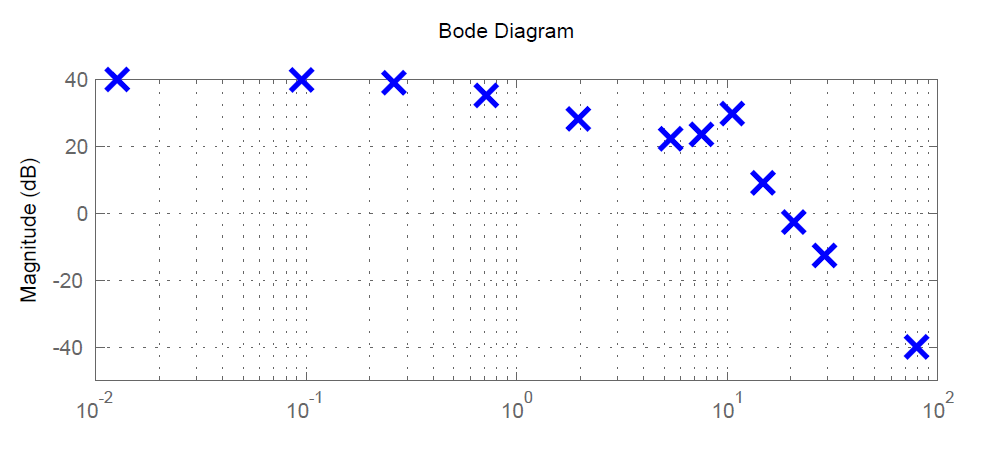
\includegraphics[width=8cm]{bilder/ident_bode.png}
\end{minipage}

\paragraph{Discrete-Time Case}
If the signals $u$ and $y$ are sampled at times $t = kT$, an input
$u(kT) = A \cdot \sin(\omega_0 k T)$
will create the expected output signal
\[
    \hat{y}(kT) = B \cdot \sin(\omega_0 k T + \varphi) 
    = B_c \cdot \cos(\omega_0 k T) + B_s \cdot \sin(\omega_0 k T)
\]
where $B = \sqrt{B_c^2 + B_s^2}$ and $\varphi = \arctan\frac{B_c}{B_s}$.
The sample time $T$ and the number of samples $N$ are chosen to be $T \cdot N = \frac{2\pi}{\omega_0}$.
Then the $B_c$ and $B_s$ which minimize the quadratic cost function reduce to
\begin{align*}
    B_c &= \frac{2}{N}\sum_{k=0}^{N-1} y(kT) \cos(2\pi lk/N) &
    B_s &= \frac{2}{N}\sum_{k=0}^{N-1} y(kT) \sin(2\pi lk/N)
\end{align*}
from which the values $B$ and $\varphi$ can be calculated.
This results in one point of the frequency response $B/A \cdot e^{j\varphi}$.

\subsubsection{Several Frequencies at Once}
The formulas for $B_c$ and $B_s$ are similar to the DFT, which is given by
\[
    \operatorname{DFT}\{f(kT)\} = F_n = \sum_{k=0}^{N-1} f(kT) e^{-j2\pi nk/N}
\]
where $F_n = F(\frac{2\pi n}{NT})$ is the frequency component at the frequency $\omega = \frac{2\pi n}{NT}$.
Using e.g. white noise or chirp signals as input signal $u$, one can calculate the frequency response by
\[
    G_d(e^{j\omega_0 T}) = \frac{\operatorname{DFT}\{y(kT)\}}{\operatorname{DFT}\{u(kT)\}} = \frac{B_s + jB_c}{A}
\]

\subsubsection{Further Nonparametric Methods}

\paragraph{Impulse Response} A discrete-time impulse at the input leads to:
\begin{align*}
    u(kT) &= \begin{cases}
        A & k=0 \\ 0 & k \neq 0
    \end{cases}
    & \Rightarrow &&
    y(kT) &= A \cdot g_d(kT) + v(kT)
\end{align*}
where $v$ is a disturbance and $g_d(kT)$ is the discrete impulse response of the system.

\paragraph{Step Response} A discrete-time step at the input leads to:
\begin{align*}
    u(kT) &= \begin{cases}
        A & k \geq 0 \\ 0 & k < 0
    \end{cases}
    & \Rightarrow &&
    y(kT) &= A \cdot \sum_{m=0}^{k} g_d(mT) + v(kT)
\end{align*}
which allows the estimation of $\hat{g}_d(kT) = \frac{y(kT) - y((k-1)T)}{A}$.

\paragraph{Deconvolution of Output} The output is a convolution of the input $u$ with the
impulse response $g_d$, i.e.
\begin{align*}
    y(0) &= g_d(0) u(0) &
    y(T) &= g_d(0) u(T) + g_d(T) u_0) &
    y(2T) &= g_d(0)u(2T) + g_d(T)u(T) + g_d(2T)u(0) &
    \dots
\end{align*}
If no disturbance $v$ is present, this can be recursively solved for $g_d$ by
\begin{align*}
    \hat{g}_d(0) &= \frac{y(0)}{u(0)} &
    \hat{g}_d(T) &= \frac{y(T) - \hat{g}_d(0)u(T)}{u(0)} = \frac{y(T)u(0) - y(0)u(T)}{u(0)^2} &
    \dots
\end{align*}

\paragraph{Effects of Nonlinearities}
These techniques are \emph{only} applicable to LTI systems.

\subsection{Parametric Identification}
A general model for SISO systems with disturbance $e(k)$ is given by
\[
    A(q) \cdot y(k) = \frac{B(q)}{F(q)} \cdot u(k) + \frac{C(q)}{D(q)}\cdot e(k)
\]
Some often used special cases are:
\begin{align*}
    A(q) \cdot y(k) &= B(q) \cdot u(k) + e(k) & \text{ARX, autoregressive} \\
    A(q) \cdot y(k) &= B(q) \cdot u(k) + C(q) \cdot e(k) & \text{ARMAX, autoregressive moving average} \\
    y(k) &= \frac{B(q)}{F(q)} \cdot u(k) + \frac{C(q)}{D(q)} \cdot e(k) & \text{BJ, Box-Jenkins} \\
    y(k) &= \frac{B(q)}{F(q)} \cdot u(k) + e(k) & \text{OE, output error}
\end{align*}

\subsection{Identifiability}
As example, consider an electromechanical system which is given by
\[
    G(s) = \frac{\frac{K_P K_{\mu} f \Phi}{R J_{\alpha} J_{\beta}}}
    {s^3 + \frac{\Phi^2}{R J_{\alpha}} s^2 + \frac{f(J_{\alpha}+J_{\beta})}{J_{\alpha}+J_{\beta}}s + \frac{f \Phi^2}{R J_{\alpha} J_{\beta}}}
    =
    \frac{b_0}{s^3 + a_2 \cdot s^2 + a_1 \cdot s + a_0}
\]
While the parameter vector $\theta_1 = [a_0 \; a_1 \; a_2 \; b_0]^T$
is \emph{identifiable}, the parameter vector
$\theta_2 = [f \; J_{\alpha} \; J_{\beta} \; \Phi \; R \; K_P \; K_{\mu}]^T$
is \emph{not}, as the model only has five independent matrix entires.
Additional knowledge, e.g. from a datasheet is needed.

\subsubsection{Basics of Least Squares (LS)}
Least squares minimizes the sum of squared errors.
It is used if equations are linear in the parameters $\theta_i$ (l.i.p.).
A form $y = f(u) = \sum_i \theta_i \cdot f_i(u)$ is l.i.p. even if the functions
$f_i(u)$ are nonlinear.

A system of linear equations $y = \Phi \theta$ is solved for $\theta$ by 
$\theta = \Phi^{-1} y$.
If the system is overdetermined, the least squares solution is
\[
    \theta = (\Phi^T \Phi)^{-1} \Phi^T y
\]

\subsubsection{Weighted Least Squares}
Introducing a weighting matrix $L$, the problem becomes $L y = L \Phi \theta$
with the solution
\[
    \theta = (\Phi^T L^T L \Phi)^{-1} \Phi^T L^T L y
\]

\paragraph{Markov Estimation by using the Covariance Matrix}
If the error term $\varepsilon$ has zero mean ($E[\varepsilon]=0$) and the
covariance matrix $V = E[\varepsilon\varepsilon^T]$ and is assumed to be
Gaussian, the optimal estimation for $\theta$ is achieved by using
$L^T L = V^{-1}$.

\subsubsection{Recursive Least Squares}
For large data collections or time-variant processes, the use of recursive methods is of interest.

Given information at time $N$,
\begin{align*}
    \theta_N &= \underbrace{(\Phi_N^T \Phi_N)^{-1}}_{P_N} \Phi_N^T y_N &
    \Phi_N &= \begin{bmatrix} \varphi_0^T \\ \vdots \\ \varphi_N^T \end{bmatrix} &
    y_N &= \begin{bmatrix} y(0) \\ \vdots \\ y(N) \end{bmatrix}
\end{align*}
with
\[
    \varphi_k^T = \begin{bmatrix}
    -y(k-1) & \dots & -y(k-n) & u(k-1) & \dots & u(k-m)
    \end{bmatrix}
\]
the new values at time $N+1$ are found by the recursive formulas
\begin{align*}
    \theta_{N+1} &= \theta_N + \frac{P_N \varphi_{N+1}}{1 + \varphi_{N+1}^T P_N \varphi_{N+1}}\left( y(N+1) - \varphi_N^T \theta_N \right) \\
    P_{N+1} &= P_N - \frac{P_N \varphi_{N+1} \varphi_{N+1}^T P_N}{1 + \varphi_{N+1}^T P_N \varphi_{N+1}}
\end{align*}

\paragraph{Forgetting Factor}
In a slowly time-variant system, old measurements should be forgotten gradually. 
This is achieved by using a \emph{forgetting factor} $\lambda\in]0,1]$ 
(typical values: $0.9 < \lambda < 0.98$) and
\[
    V^{-1} = L^T L = \begin{bmatrix}
        \lambda^N & 0 &\dots & 0 \\
        0 & \ddots & \ddots & \vdots \\
        \vdots & \ddots & \lambda & 0 \\
        0 & \dots & 0 & 1
    \end{bmatrix}
\]
Which leads to the recursive formulas
\begin{align*}
    \theta_{N+1} &= \theta_N + \frac{P_N \varphi_{N+1}}{\lambda + \varphi_{N+1}^T P_N \varphi_{N+1}}\left( y(N+1) - \varphi_N^T \theta_N \right) \\
    P_{N+1} &= \frac{1}{\lambda} \cdot \left(P_N - \frac{P_N \varphi_{N+1} \varphi_{N+1}^T P_N}{\lambda + \varphi_{N+1}^T P_N \varphi_{N+1}}\right)
\end{align*}

\subsection{Practical Aspects of Identification}

\paragraph{Identificatoin Cycle}The identification process is an iterative task.
\paragraph{Sampling Time}An anti-aliasing filter $G_{f}$ must be applied to the analog signal.
\paragraph{Identification of Closed-Loop Systems} A plant might be unstable or
in use for production, or it might contain some built-in feedback mechanisms.
Then the plant has to be identified in a closed loop.